
\chapter{Uživatelské testování}

Uživatelské testování prováděl tester za přítomnosti mé a mého kolegy z~týmu. Jeho hlavním účelem bylo najít chyby v~programu, na které jsem sám nepřišel. V~této kapitole popisuji pouze testování těch částí systému, které jsem sám programoval. Testování částí, které dělal kolega, zde nepopisuji.



%----------------------------------------------------------------------------------------------------------

% uziv. zkusil zmenit MAC adresu - chyba
% ifconfig --help vypsal chybu, at uzivatel zkusi ifconfig --help
% ping -c 4 192.168.1.1 - chyba -mezera mezi 'c' a 4
% ping IP prepinace - nefunguje
% man route nefunguje
% route -h a --help a --version nefunguje
% prepsat vypisy z Cj do Aj 
% echo 1 > ip_forward - ma tam byt jen /proc/sys/net/..


\section{Průběh testování}


\subsection{Spuštění aplikace}

Prvním úkolem testera bylo aplikaci spustit a zjistit, jak se s~ní zachází. Toto činilo uživateli menší problémy, protože chybová hlášení vyhazovaná simulátorem nebyla dost jasná na to, aby uživatel pochopil, jak se má chyb vyvarovat. Spouštění aplikace je práce mého kolegy a ten chyby opravil.


\subsection{Práce s~aplikací}

Tester měl za úkol zkonfigurovat síť z obrázku \ref{obr_testovani}. Během konfigurace přišel na chyby, které zde popisuji, a zároveň také popisuji, jak byly opraveny.

% testovací síť
\begin{figure}[h]
\begin{center}
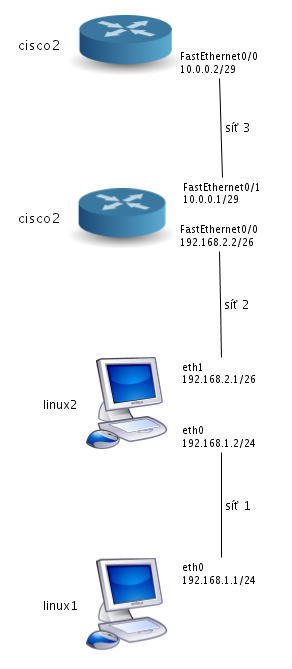
\includegraphics[width=5cm]{obrazky/testovani}
\caption{Testovací síť, kterou tester konfiguroval}
\label{obr_testovani}
\end{center}
\end{figure}

\subsubsection{Výpisy}

Hlášení o~běhu simulátoru, která jsou vypisována na standardní výstup, se testerovi zdála velmi nepřehledná. Výpisy o~tom, co server posílá jednotlivým klientům a co klienti posílají serveru, jsou pro uživatele nadbytečné a proto byly zrušeny. Ponechány byly jen výpisy o~přihlášení klienta a o~průchodu paketu, které byly testerovi užitečné pro diagnostiku sítě.

\subsubsection{Příkaz ifconfig}

Tester zkoušel změnit mac adresu rozhraní, což simulátor nepodporuje. Přidal jsem příkaz \verb|help|, který popisuje, jaké varianty příkazů jsou podporovány.

Tester zkoušel příkaz \verb|ifconfig --help|, který nefunguje. Chybu jsem opravil.

\subsubsection{Manuálové stránky}

Tester zkusil zadat \verb|man route|, přičemž simulátor vypsal, že příkaz neexistuje. Dodělal jsem příkaz \verb|man|, který vypíše, že manuálové stránky nejsou implementovány a doporučí uživateli příkaz \verb|help|.

\subsubsection{Příkaz ping}

Uživatel zadal příkaz \verb|ping 192.168.1.1 -c5|. Zjistil, že parametr \verb|-c| je ignorován, protože parser parsuje jen parametry před adresou. Parser jsem z důvodu veliké časové tísně zatím nestihl opravit. Chyba je zmíněna přímo u popisu tohoto příkazu a bude opravena.

\subsubsection{Soubor ipforward}

Z důvodů snazšího testování jsem měl na soubor \verb|/proc/sys/net/ipv4/ip_forward| nastaven alias \verb|ip_forward|, který jsem zapomněl odstranit. Alias již byl odstraněn.

\subsubsection{Příkaz route}

Tester zkoušel příkaz \verb|route --help|, který nefunguje. Do parseru jsem přidal parsování tohoto přepínače.



%----------------------------------------------------------------------------------------------------------

\section{Závěr}

V aplikaci bylo nalezeno několik, spíše drobnějších chyb především v parsování příkazů. Některé chyby již byly opraveny, některé teprve opravím a jistě existují chyby, zvláště v parserech, které ještě nebyly nalezeny. Ty budu muset opravit, až na ně uživatelé, budou-li kdy nějací, přijdou.

V simulátoru nebyly nalezeny žádné vážnější chyby v jeho datových strukturách a ve virtuální síti. Nebyly nalezeny ani žádné chyby, které by způsobovaly pád naší aplikace.
